%==============================================================================
% CHAPTER 5 --- SYSTEM IMPLEMENTATION
%==============================================================================

\chapter{System Implementation}
\label{chap:implementation}

\chapterquote{The best designs are those that successfully become working systems.}{Alan Kay}

%==============================================================================
\section{Overview}
\label{sec:implementation_overview}

This chapter presents the implementation details of the proposed NABTA platform. Following the system methodology presented in Chapter~3 and the architectural design described in Chapter~5, this chapter demonstrates how the proposed solution was transformed into a fully functional smart agriculture platform.

The implementation integrates modern web technologies, deep learning models, machine learning algorithms, cloud services, and explainable artificial intelligence within a unified production-ready application. The platform consists of a React.js frontend, a FastAPI backend, multiple AI models for image analysis and agricultural recommendation, Firebase cloud services, and a Retrieval-Augmented Generation (RAG) chatbot powered by the Cohere API.

The implementation workflow follows the same sequence adopted by the deployed system. First, the graphical user interfaces are presented, followed by the backend implementation, AI model integration, cloud services, and finally the complete system workflow.

%==============================================================================
\section{Frontend Implementation}
\label{sec:frontend}

The frontend of NABTA was implemented using React.js as a Single-Page Application (SPA). The interface was designed to provide an intuitive user experience while supporting complex AI functionalities through a modern dashboard-based design.

Responsive layouts, reusable components, dark/light themes, interactive visualizations, and asynchronous communication with the backend enable users to access all platform services through a unified interface.

The following subsections present the main user interfaces implemented in the system.

%==============================================================================
\subsection{Home Page}
\label{subsec:landing}

The landing page serves as the public entry point to the NABTA platform. It introduces the objectives of the system, highlights the available artificial intelligence services, and provides quick access to authentication and analysis modules.

The page presents the major capabilities of the platform, including plant disease diagnosis, crop recommendation, irrigation management, AI-powered consultation, and analytical dashboards. Modern animations and responsive design techniques were adopted to improve usability across desktop and mobile devices.

\begin{figure}[H]
\centering
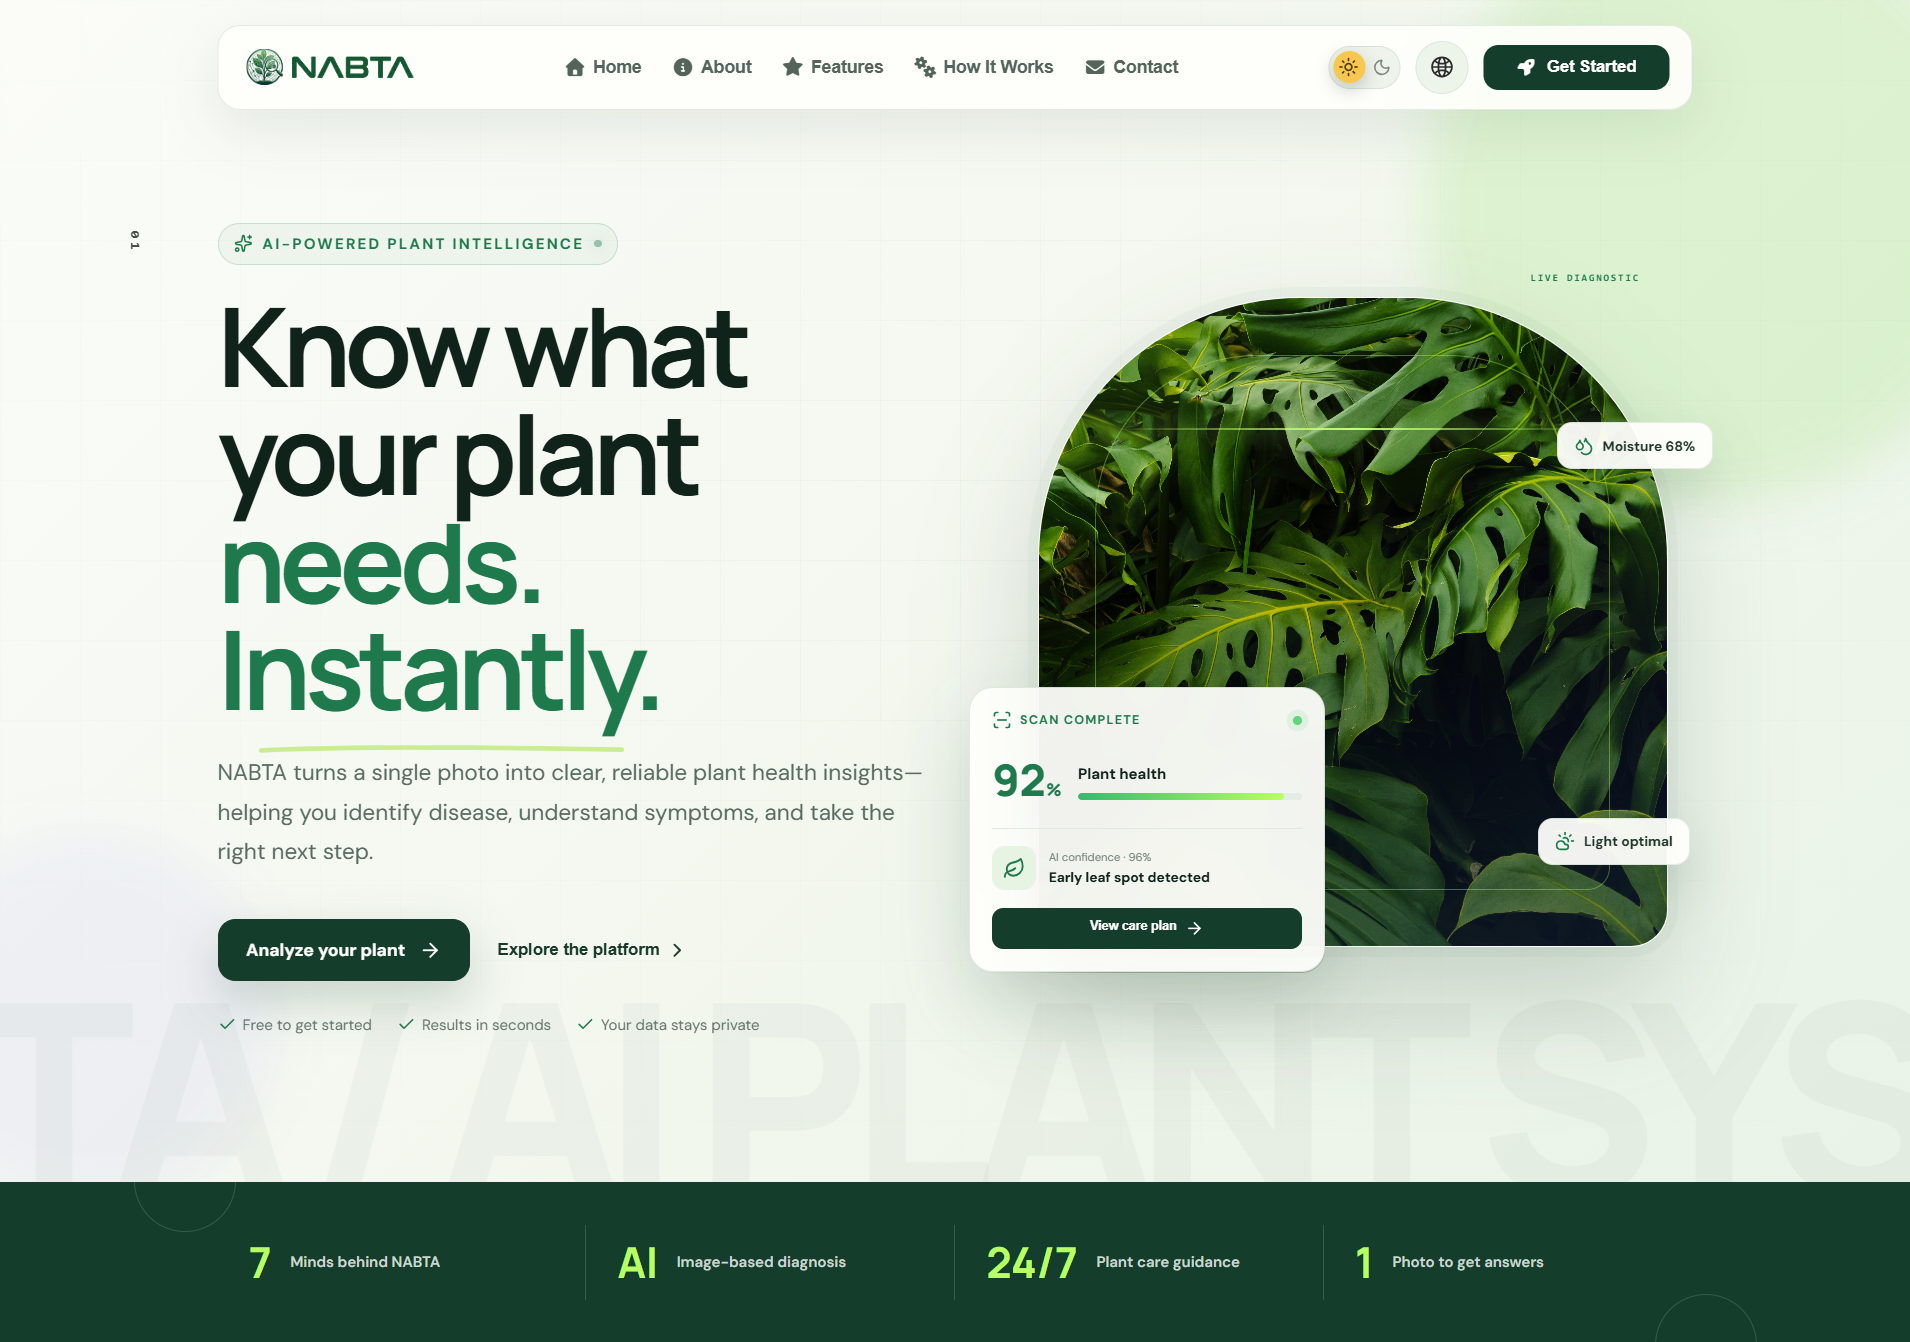
\includegraphics[width=\textwidth]{assets/screenshots/home_page.png}
\caption{NABTA Landing Page}
\label{fig:landing_page}
\end{figure}

%==============================================================================
\subsection{User Authentication}
\label{subsec:login}

User authentication is implemented using Firebase Authentication, providing secure account management through email and password authentication.

The authentication interface validates user credentials before granting access to protected platform features. Authentication tokens are securely generated by Firebase and verified by the FastAPI backend before processing any authorized request.

The login page also provides direct navigation to account registration and password recovery services.

\begin{figure}[H]
\centering
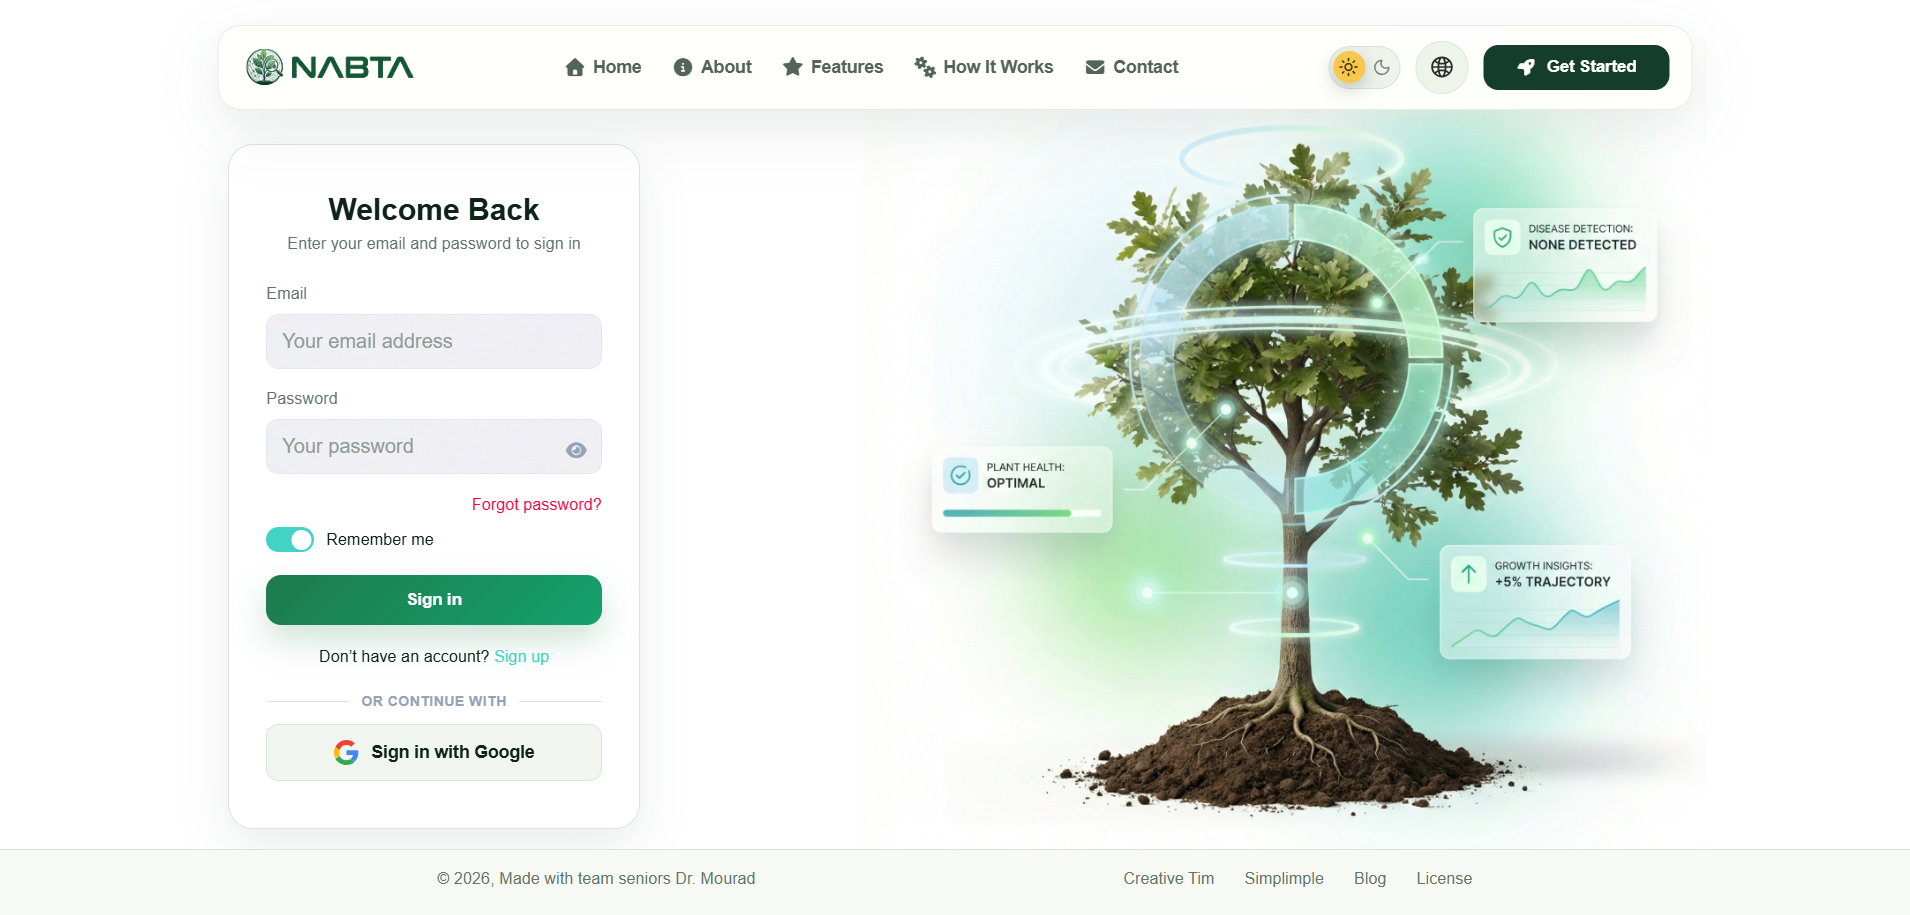
\includegraphics[width=.9\textwidth]{assets/screenshots/login_page.png}
\caption{User Authentication Interface}
\label{fig:login_page}
\end{figure}

%==============================================================================
\subsection{Password Recovery}
\label{subsec:reset_password}

To improve usability and account security, NABTA provides a password recovery mechanism integrated with Firebase Authentication.

Users can request a password reset by entering their registered email address. A secure password reset link is then sent automatically, allowing users to create a new password without administrator intervention.

This functionality improves accessibility while maintaining secure account management practices.

\begin{figure}[H]
\centering
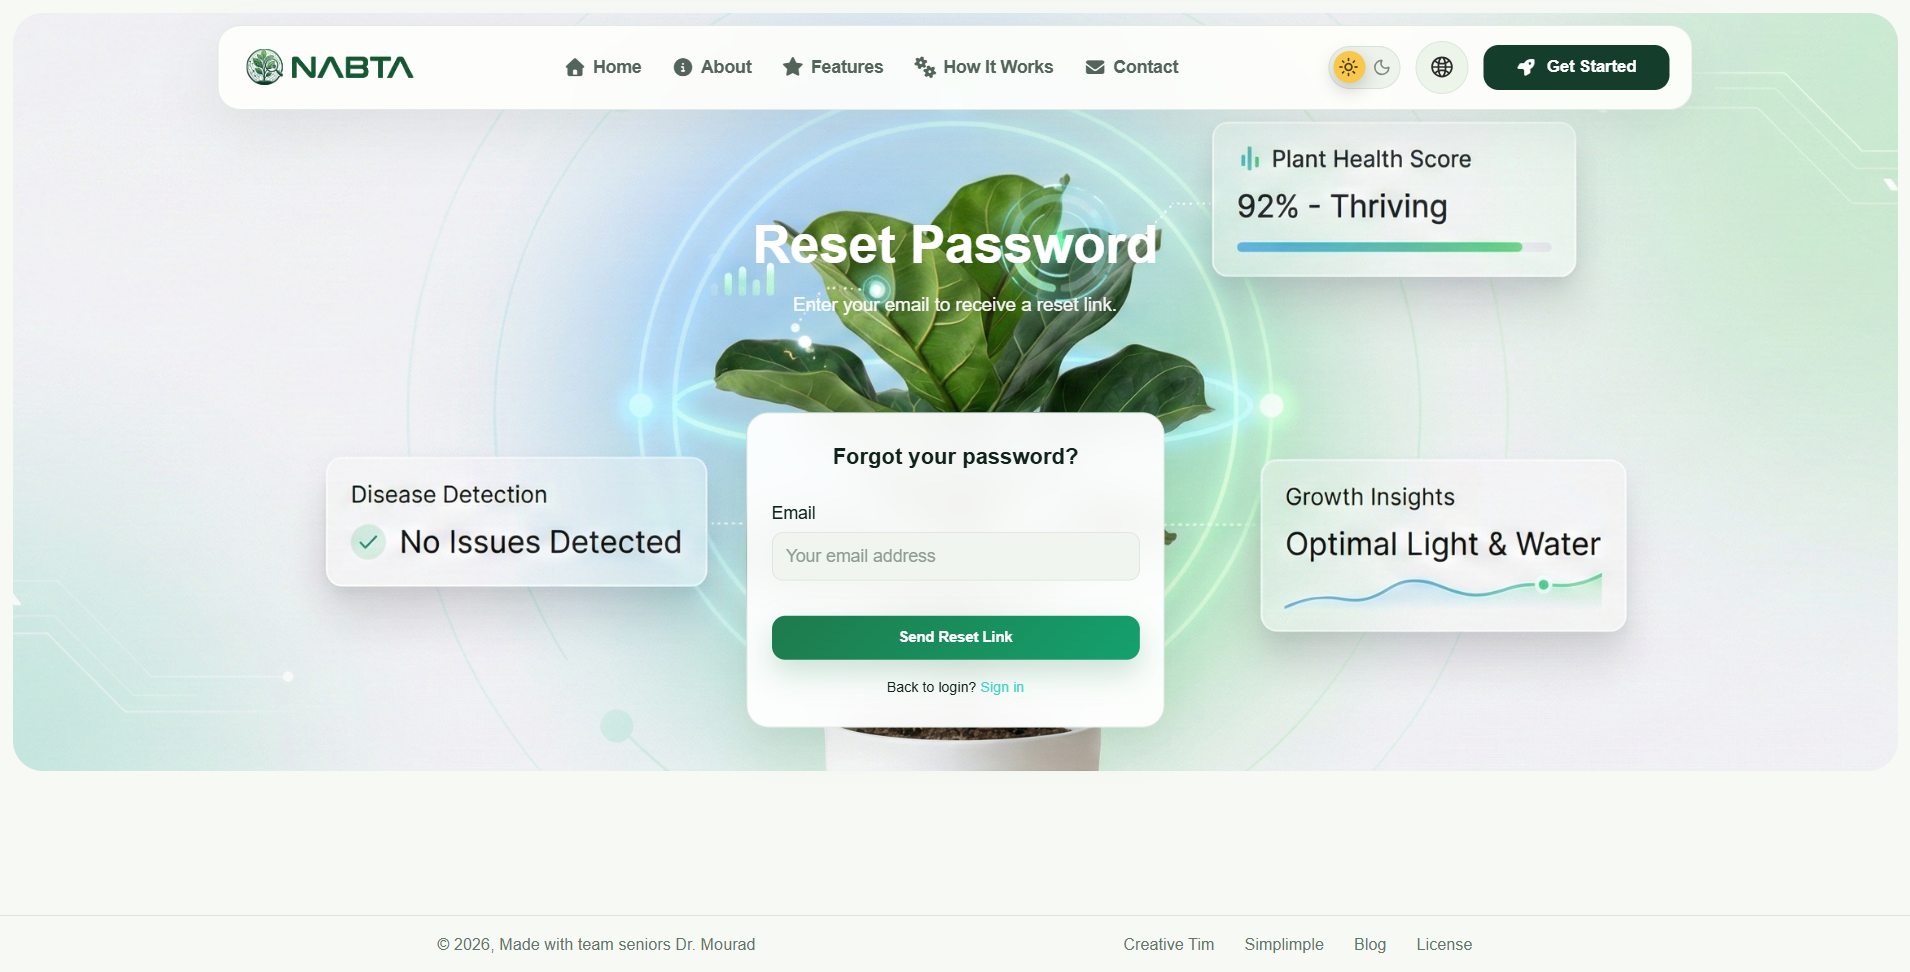
\includegraphics[width=.85\textwidth]{assets/screenshots/reset_password.png}
\caption{Password Recovery Interface}
\label{fig:reset_password}
\end{figure}

%==============================================================================
\subsection{Plant Analysis Interface}
\label{subsec:plant_analysis}

The Plant Analysis module represents the primary functionality of the NABTA platform. It enables users to upload plant leaf images for automatic disease diagnosis through the integrated artificial intelligence pipeline.

The interface supports drag-and-drop image uploading as well as conventional file selection. Before processing begins, the uploaded image is validated to ensure that only supported image formats are accepted.

Once the image is submitted, the frontend sends it asynchronously to the FastAPI backend, where the complete AI pipeline is executed.

\begin{figure}[H]
\centering
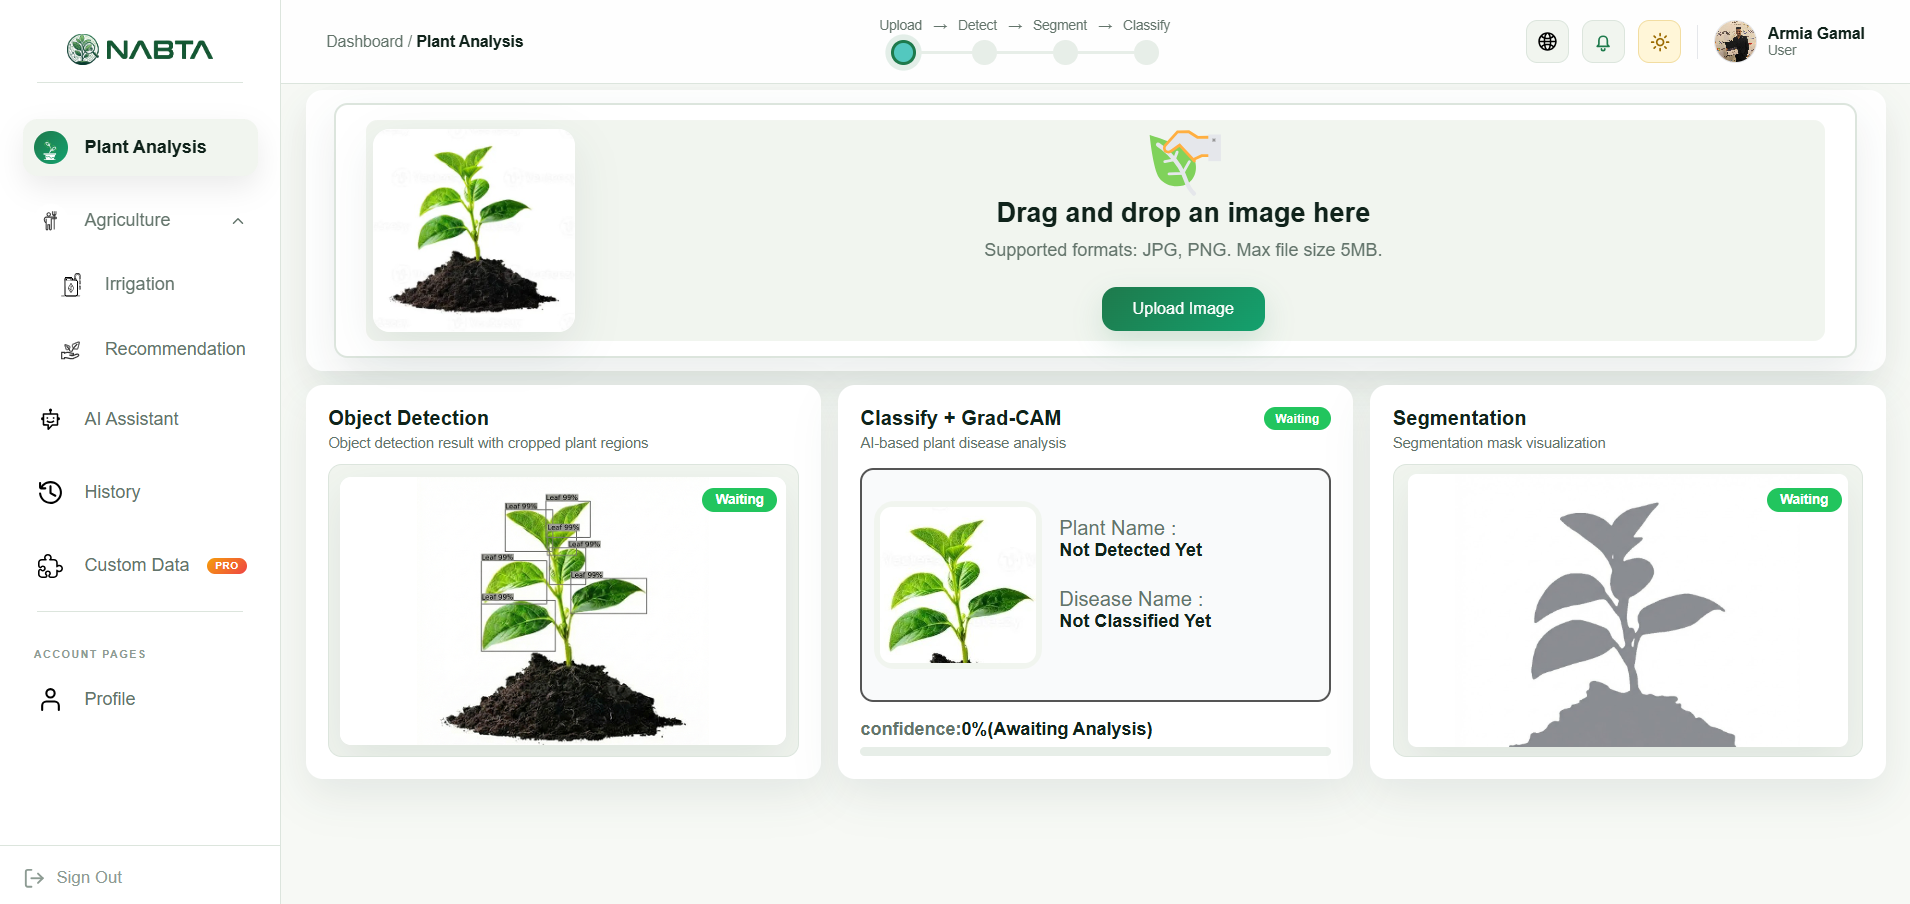
\includegraphics[width=\textwidth]{assets/screenshots/plant_analysis_upload.png}
\caption{Plant Analysis Upload Interface}
\label{fig:plant_upload}
\end{figure}

%==============================================================================
%==============================================================================
\subsection{Plant Disease Analysis Results}
\label{subsec:analysis_results}

After the uploaded image is processed, the NABTA platform presents a unified analysis interface that visualizes the complete artificial intelligence pipeline. Instead of displaying only the predicted disease, the system provides the outputs of all integrated computer vision models within a single dashboard, allowing users to understand each stage of the diagnosis process.

The interface presents:

\begin{itemize}
\item The uploaded plant image.
\item YOLOv8x object detection with the detected leaf bounding box.
\item U-Net semantic segmentation of the leaf.
\item CNN-based plant species and disease classification.
\item Prediction confidence score.
\item Disease severity estimation.
\item Direct access to the complete disease analysis report.
\end{itemize}

Displaying all analysis stages together improves transparency and enables users to verify the complete decision-making process rather than relying solely on the final prediction. This integrated visualization also demonstrates the interaction between the detection, segmentation, and classification models within the proposed NABTA pipeline.

\begin{figure}[H]
\centering
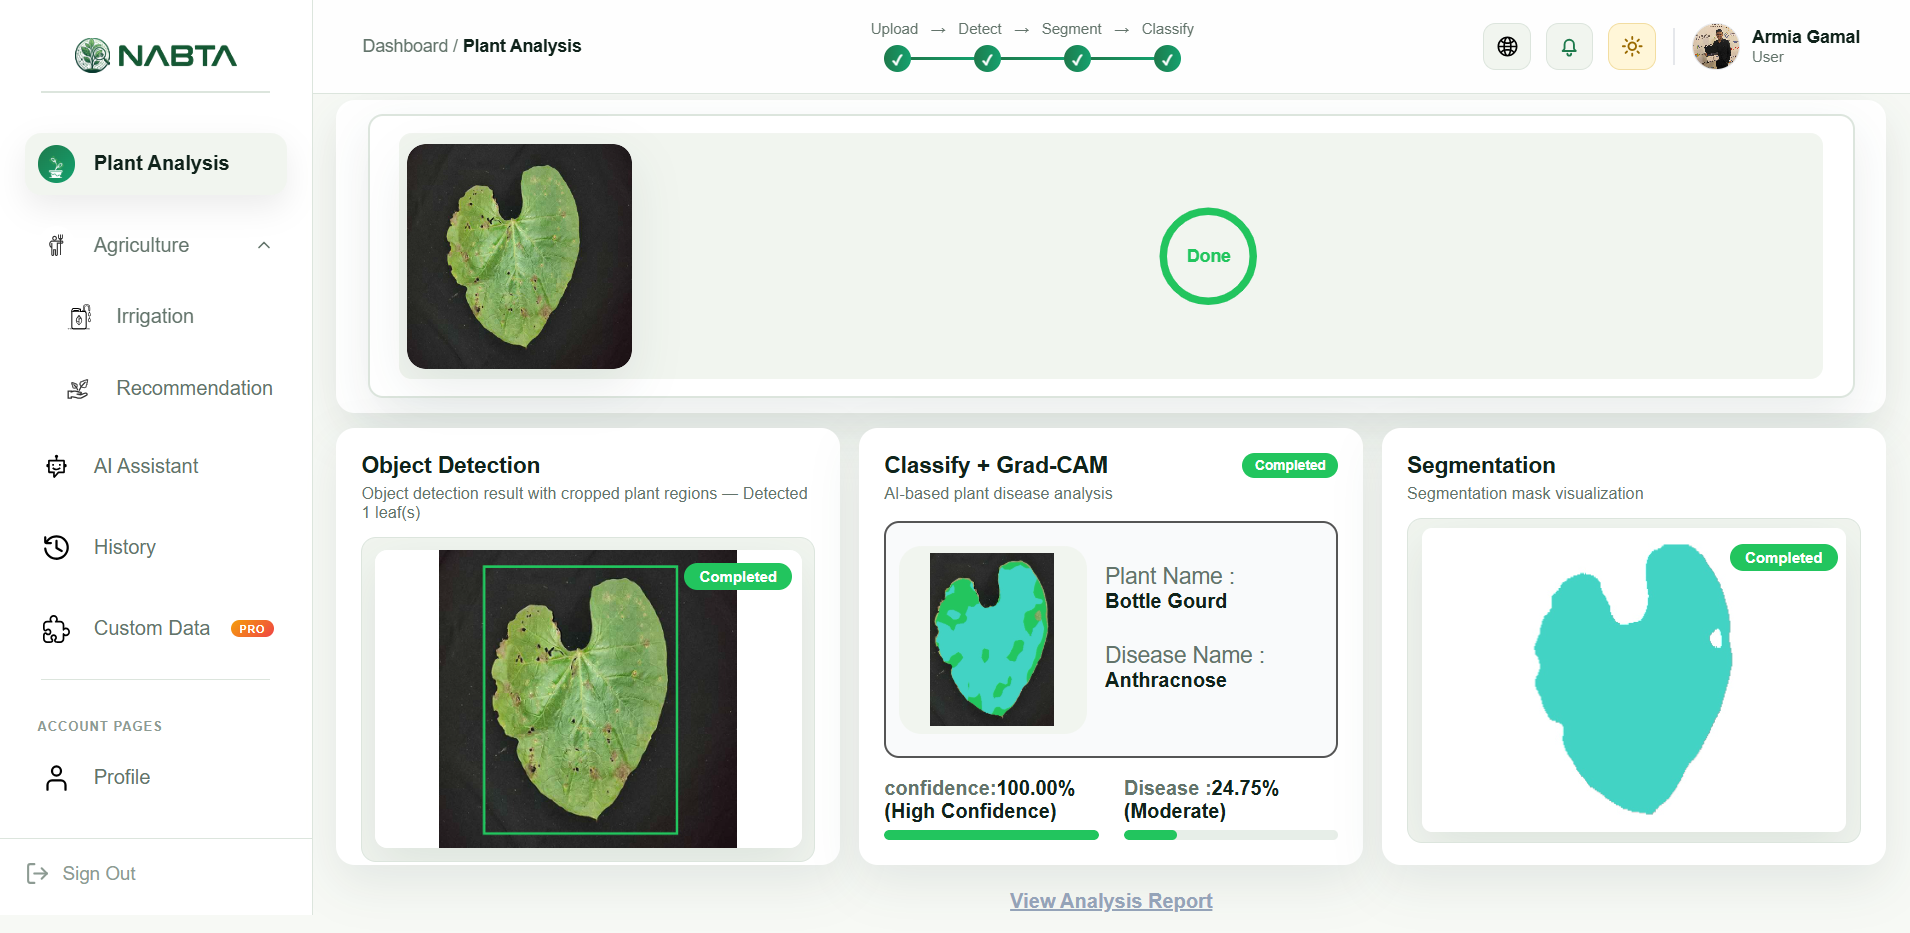
\includegraphics[width=\textwidth]{assets/screenshots/analysis_results.png}
\caption{Integrated Plant Disease Analysis Interface Showing the Outputs of YOLOv8x Detection, U-Net Segmentation, CNN Classification, Confidence Score, and Disease Severity Estimation}
\label{fig:analysis_results}
\end{figure}

%==============================================================================
\subsection{Disease Diagnosis Report}
\label{subsec:disease_report}

Following image analysis, NABTA generates a detailed disease diagnosis report summarizing all extracted information.

The report contains the predicted disease class, confidence score, detected plant species, disease severity level, Grad-CAM visualization, and recommended treatment guidelines.

This report provides users with a complete overview of the analysis outcome while serving as a basis for subsequent agricultural recommendations.

\begin{figure}[H]
\centering
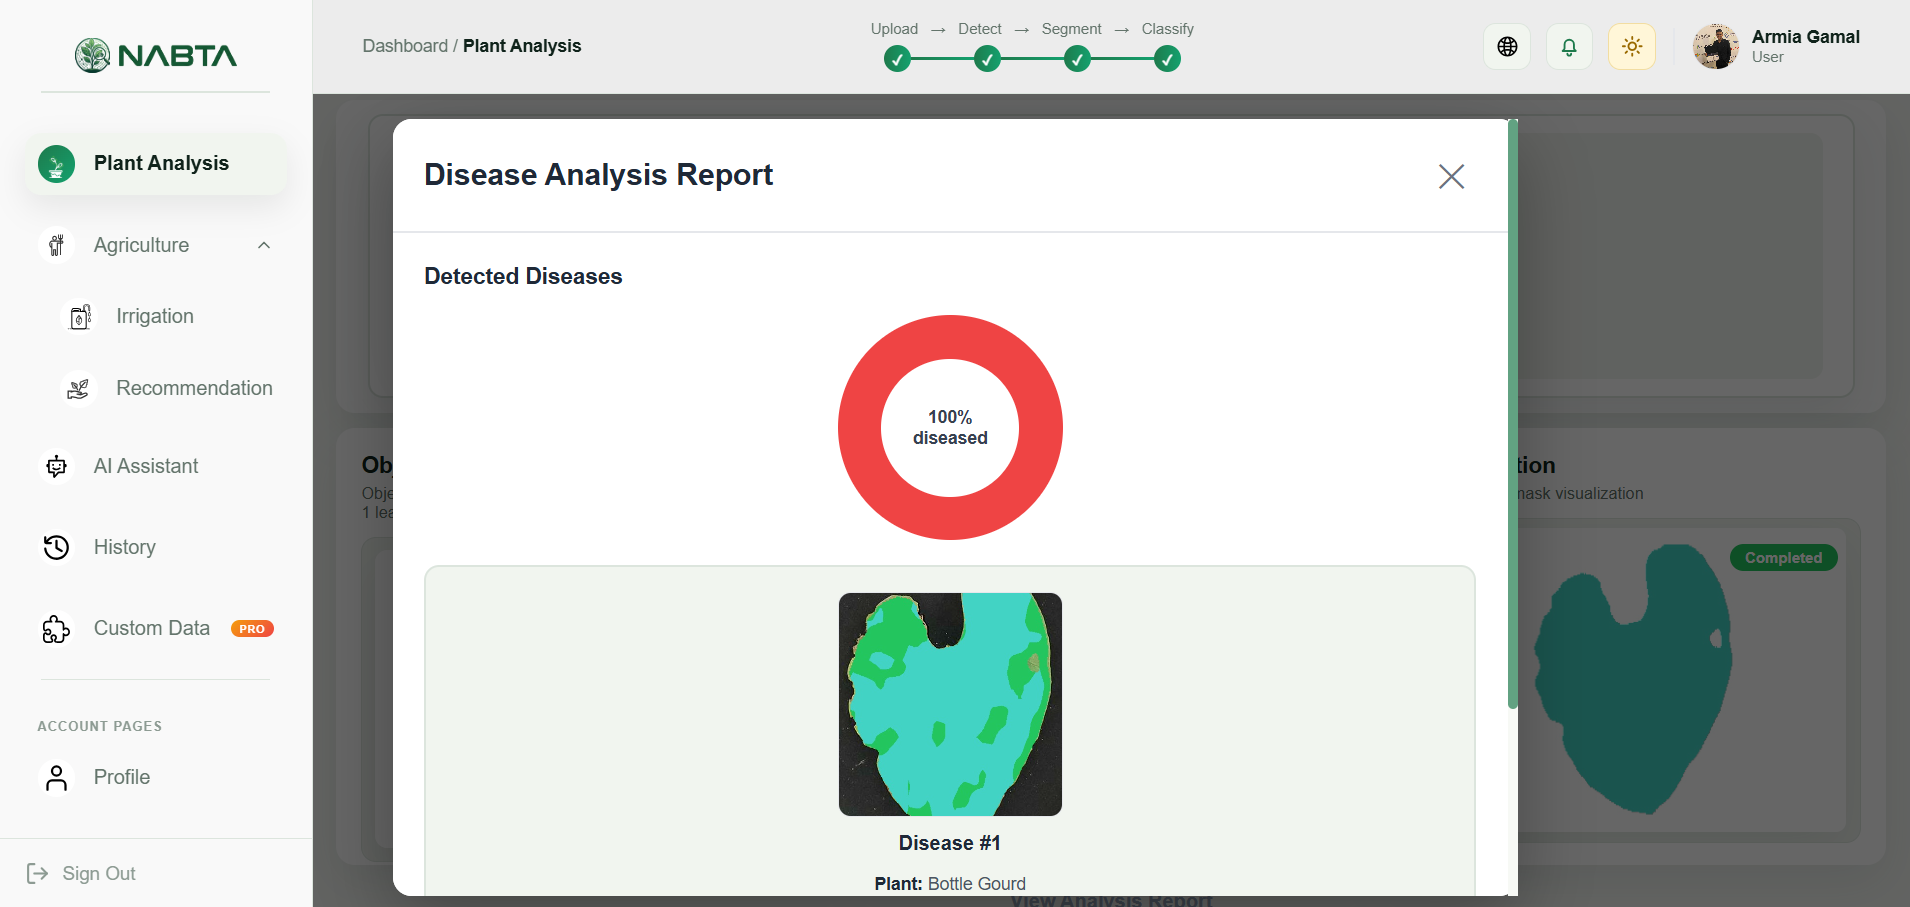
\includegraphics[width=\textwidth]{assets/screenshots/disease_report.png}
\caption{Disease Analysis Report}
\label{fig:disease_report}
\end{figure}

%==============================================================================
\subsection{AI Agricultural Assistant}
\label{subsec:assistant}

To provide intelligent agricultural consultation beyond disease diagnosis, NABTA integrates an AI-powered conversational assistant.

The assistant combines Cohere's Large Language Model with Retrieval-Augmented Generation (RAG), enabling it to retrieve domain-specific agricultural knowledge before generating responses.

Users may ask questions regarding disease symptoms, treatment methods, crop management, irrigation practices, fertilizers, and general farming recommendations.

The chatbot supports both Arabic and English, providing context-aware responses based on the retrieved agricultural knowledge base.

\begin{figure}[H]
\centering
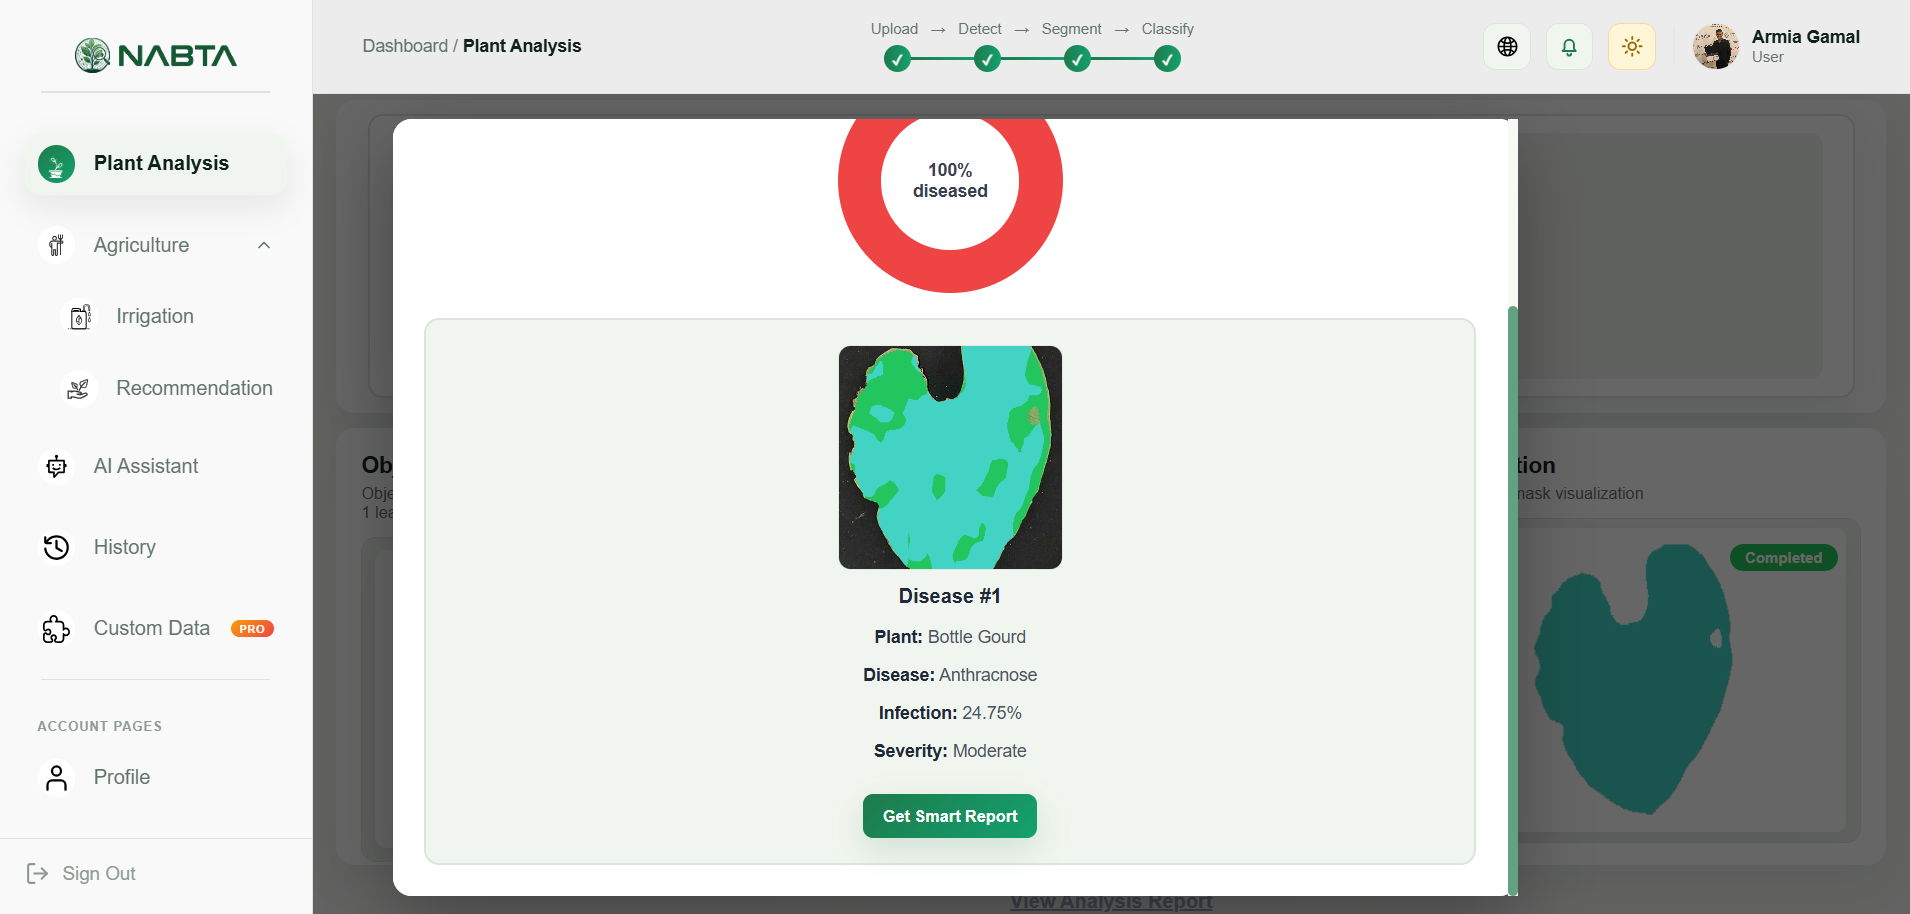
\includegraphics[width=\textwidth]{assets/screenshots/ai_assistant.png}
\caption{AI Agricultural Assistant}
\label{fig:assistant}
\end{figure}

%==============================================================================
\subsection{AI Recommendations}
\label{subsec:recommendations}

After completing the disease diagnosis process, the platform automatically generates intelligent recommendations to assist users in making informed agricultural decisions.

The recommendation engine combines the outputs of the disease classification model with the knowledge retrieved by the Retrieval-Augmented Generation (RAG) system. Based on the detected disease, the platform provides practical guidance regarding treatment methods, disease prevention strategies, suitable pesticides or fungicides, irrigation considerations, and crop management practices.

Presenting recommendations immediately after diagnosis enables users to move directly from disease identification to actionable agricultural decisions.

\begin{figure}[H]
\centering
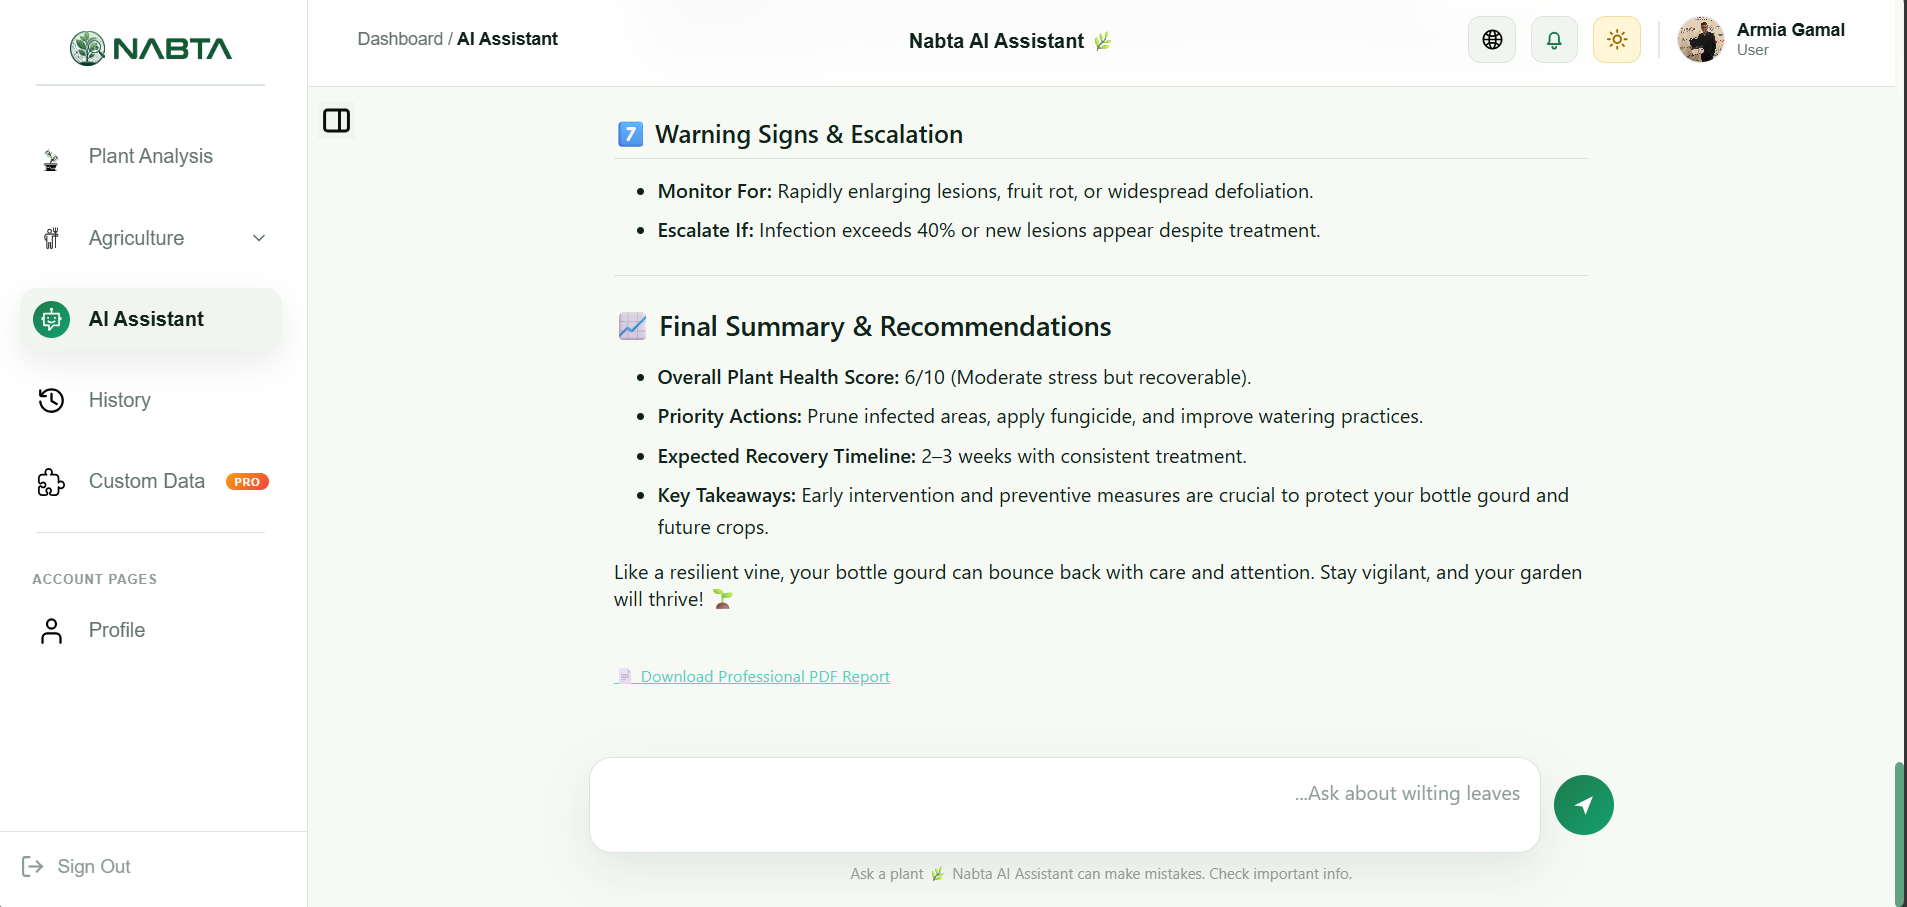
\includegraphics[width=\textwidth]{assets/screenshots/ai_recommendations.png}
\caption{AI-Based Agricultural Recommendations}
\label{fig:recommendations}
\end{figure}

%==============================================================================
\subsection{PDF Disease Report}
\label{subsec:pdf_report}

To facilitate documentation and information sharing, NABTA automatically generates a downloadable PDF report for every completed disease analysis.

The generated report summarizes all information produced during the AI pipeline, including the uploaded image, detected disease, confidence score, Grad-CAM visualization, disease severity, recommended treatment, and additional agricultural guidance.

The PDF report enables farmers, agricultural engineers, and researchers to archive diagnosis results or share them with specialists for further consultation.

\begin{figure}[H]
\centering
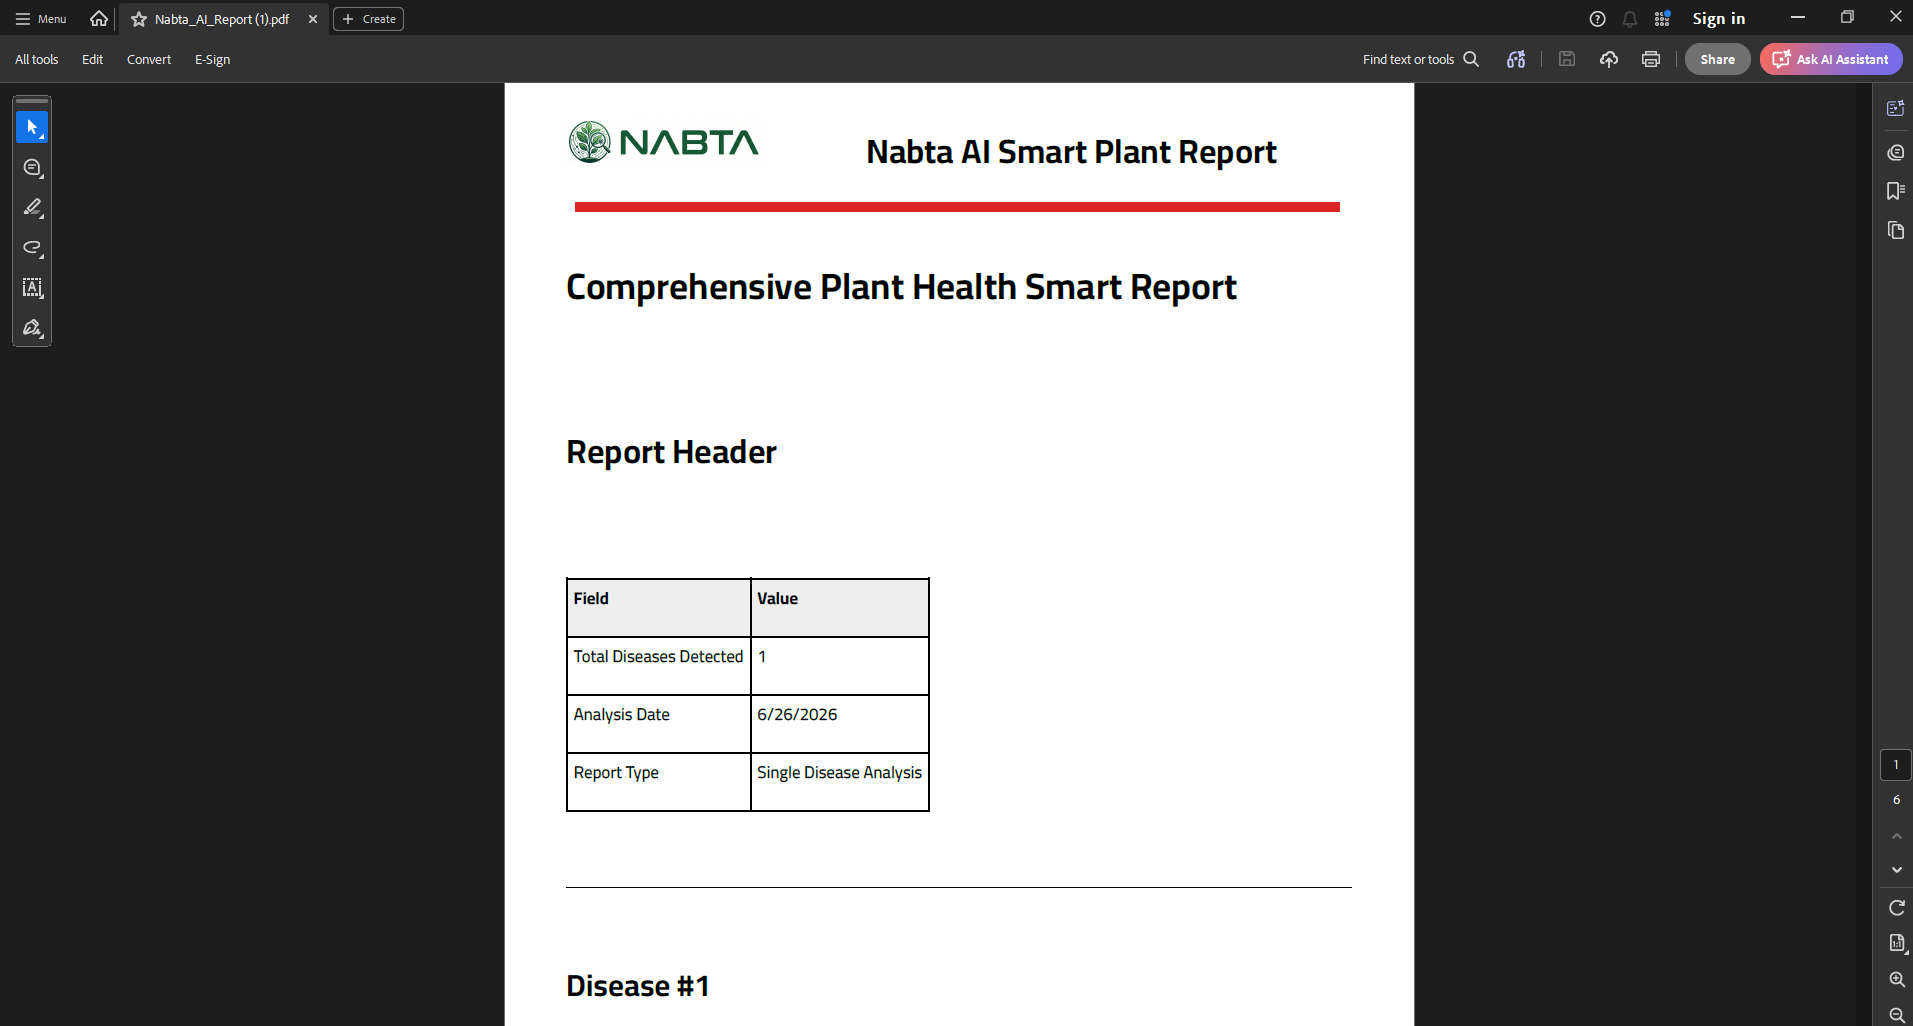
\includegraphics[width=\textwidth]{assets/screenshots/pdf_report.png}
\caption{Automatically Generated PDF Disease Report}
\label{fig:pdf_report}
\end{figure}

%==============================================================================
\subsection{Analysis Dashboard}
\label{subsec:dashboard}

The dashboard provides users with an integrated overview of their activities and the overall performance of the NABTA platform.

It summarizes important information including the total number of analyses, diagnosed diseases, healthy plant detections, generated reports, and recent AI activities. Interactive widgets and graphical indicators allow users to quickly monitor system usage and recent analysis results.

The dashboard serves as the central navigation point after user authentication.

\begin{figure}[H]
\centering
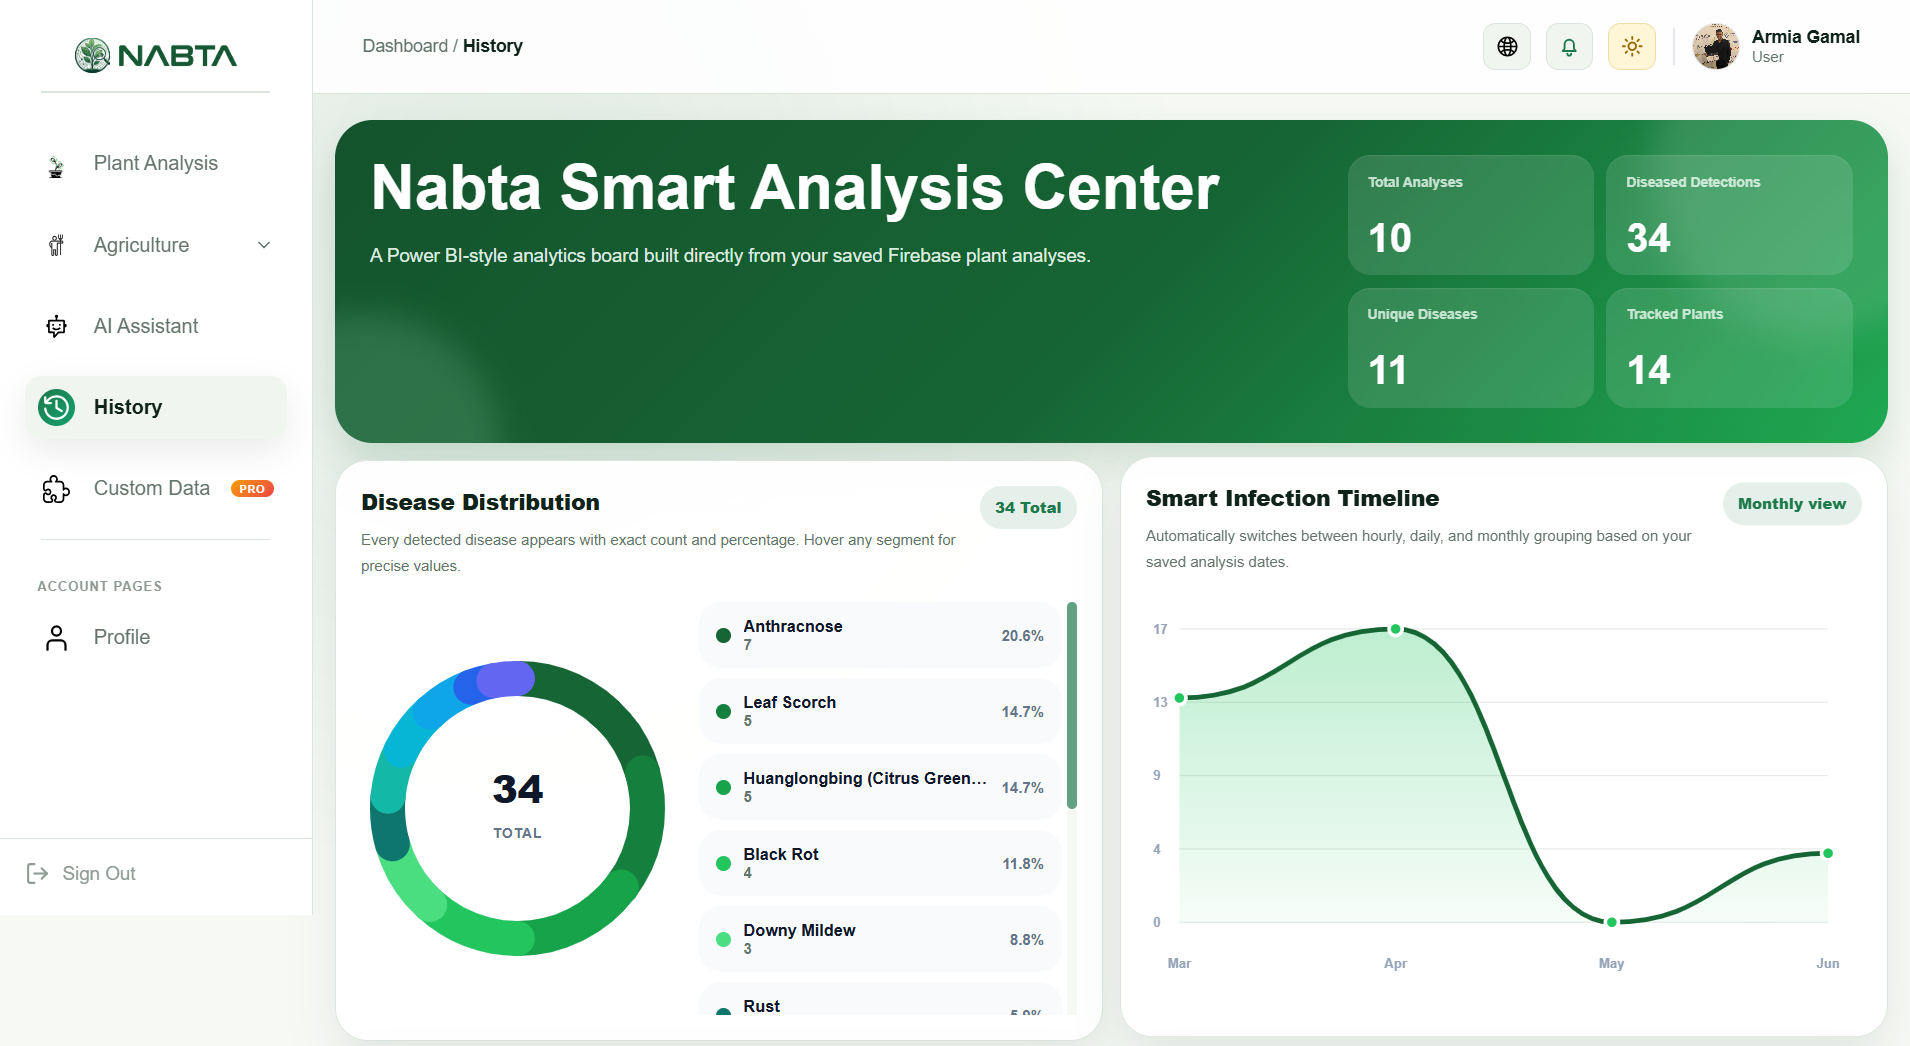
\includegraphics[width=\textwidth]{assets/screenshots/dashboard.png}
\caption{Analysis Dashboard}
\label{fig:dashboard}
\end{figure}

%==============================================================================
\subsection{Plant and Disease Analytics}
\label{subsec:analytics}

NABTA includes an analytics module that visualizes historical disease statistics and plant health trends.

Interactive charts display the distribution of detected diseases, healthy versus diseased samples, frequently analyzed plant species, confidence score distributions, and temporal analysis trends.

These visualizations assist users in understanding disease prevalence while providing useful insights for monitoring crop health over time.

\begin{figure}[H]
\centering
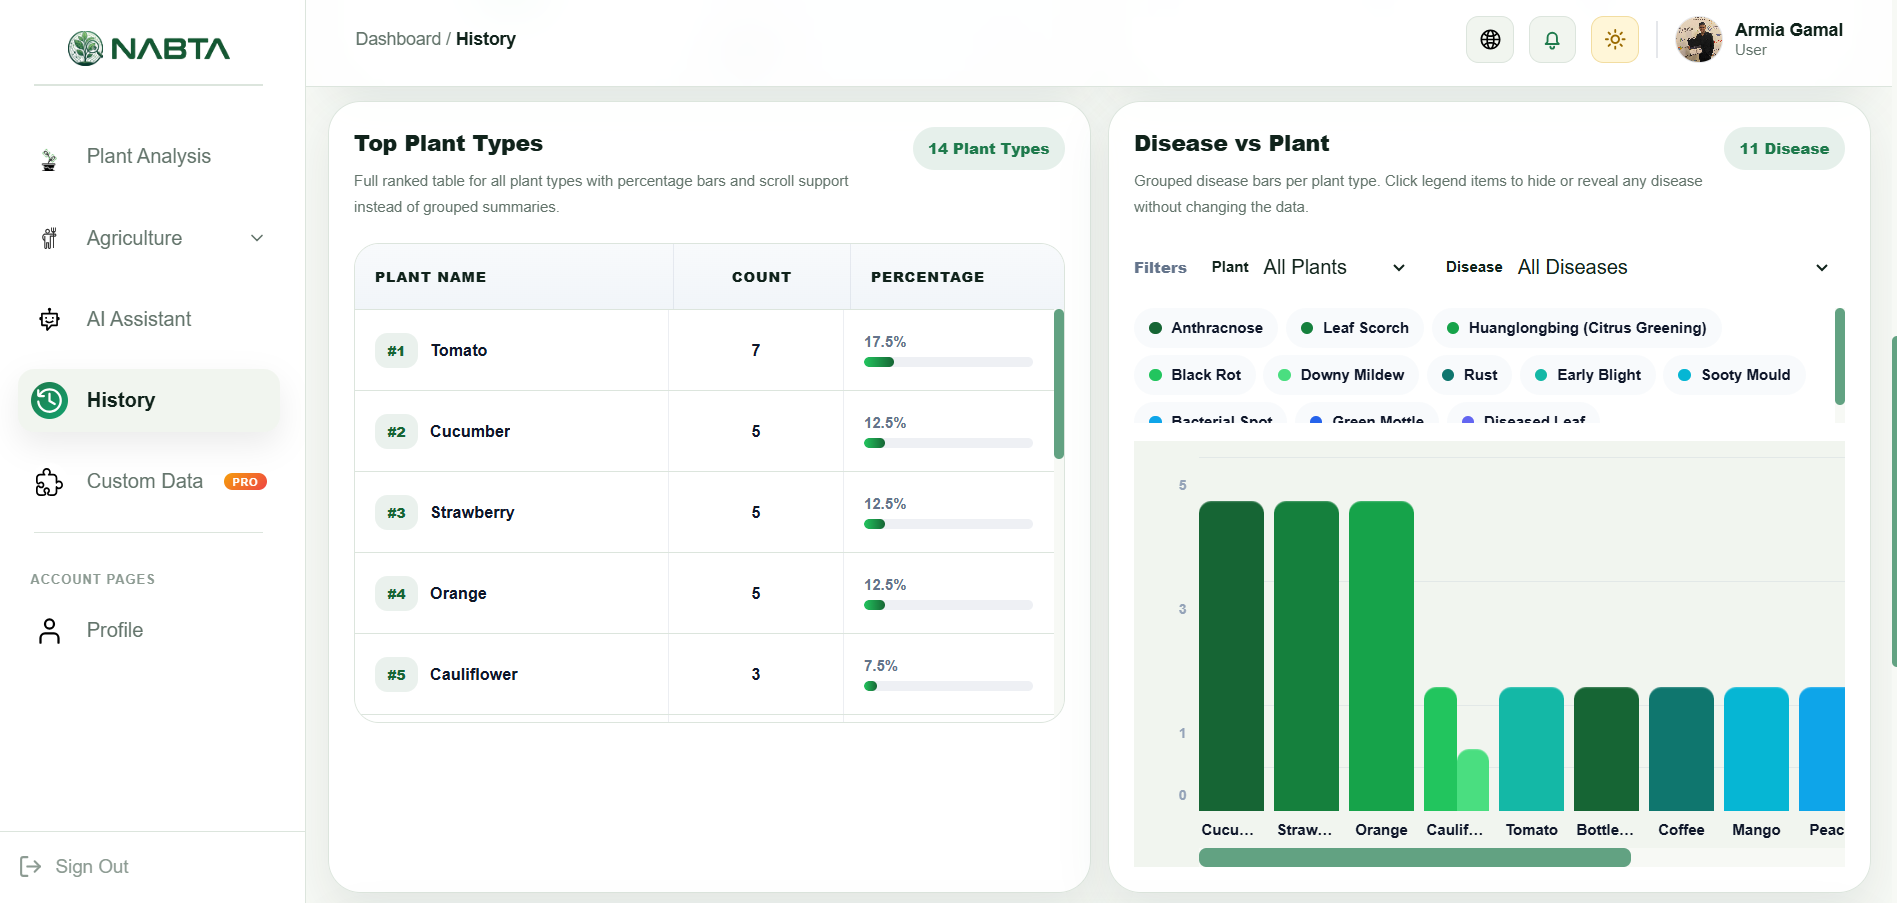
\includegraphics[width=\textwidth]{assets/screenshots/analytics.png}
\caption{Plant and Disease Analytics Dashboard}
\label{fig:analytics}
\end{figure}

%==============================================================================
\subsection{Analysis History}
\label{subsec:history}

Every completed analysis is securely stored within the user's account, allowing previous diagnoses to be reviewed at any time.

The history interface displays previously analyzed images together with their corresponding disease predictions, confidence scores, timestamps, and generated reports.

Users can search, filter, revisit, or download previous analysis reports without repeating the disease detection process.

Maintaining historical records improves traceability and enables long-term monitoring of crop health.

\begin{figure}[H]
\centering
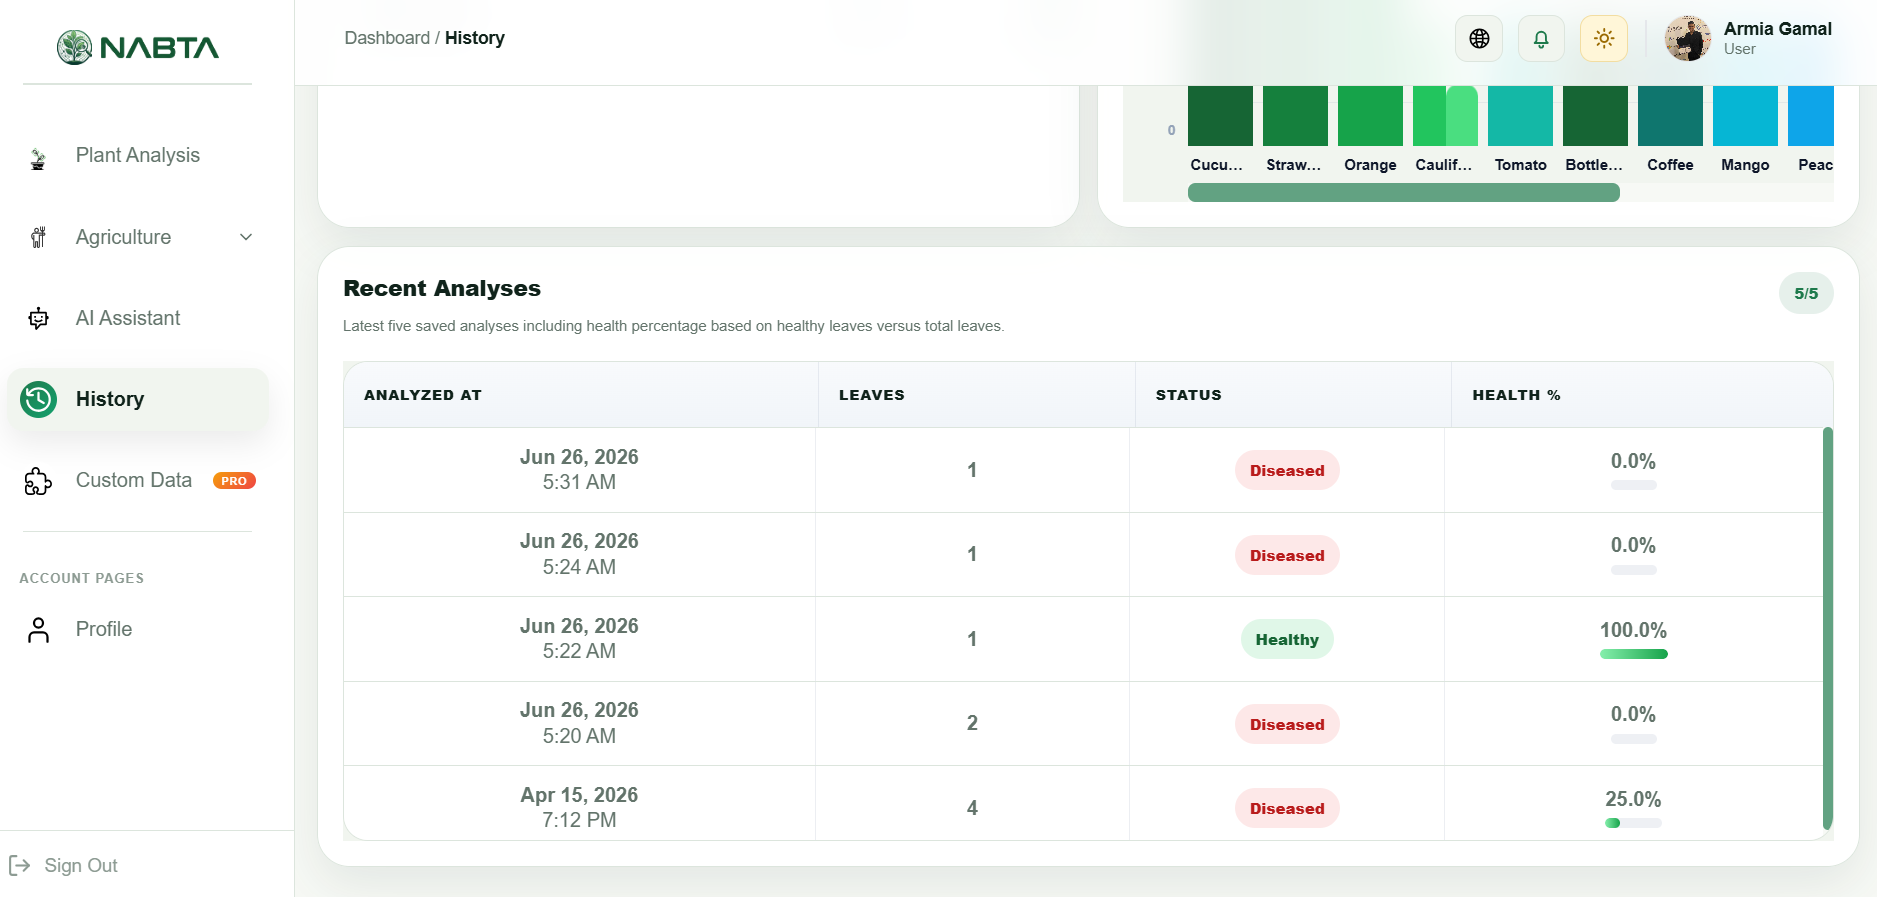
\includegraphics[width=\textwidth]{assets/screenshots/history.png}
\caption{Analysis History Interface}
\label{fig:history}
\end{figure}

%==============================================================================
\subsection{Irrigation Management}
\label{subsec:irrigation}

The irrigation management module assists farmers in making informed irrigation decisions using machine learning models trained on agricultural and environmental data.

Users provide soil moisture, soil type, crop type, temperature, humidity, rainfall, and other environmental parameters. The platform then predicts whether irrigation is required and estimates the expected crop water requirement.

The interface presents the prediction results in a clear and user-friendly format, enabling farmers to optimize irrigation schedules while reducing unnecessary water consumption.

\begin{figure}[H]
\centering
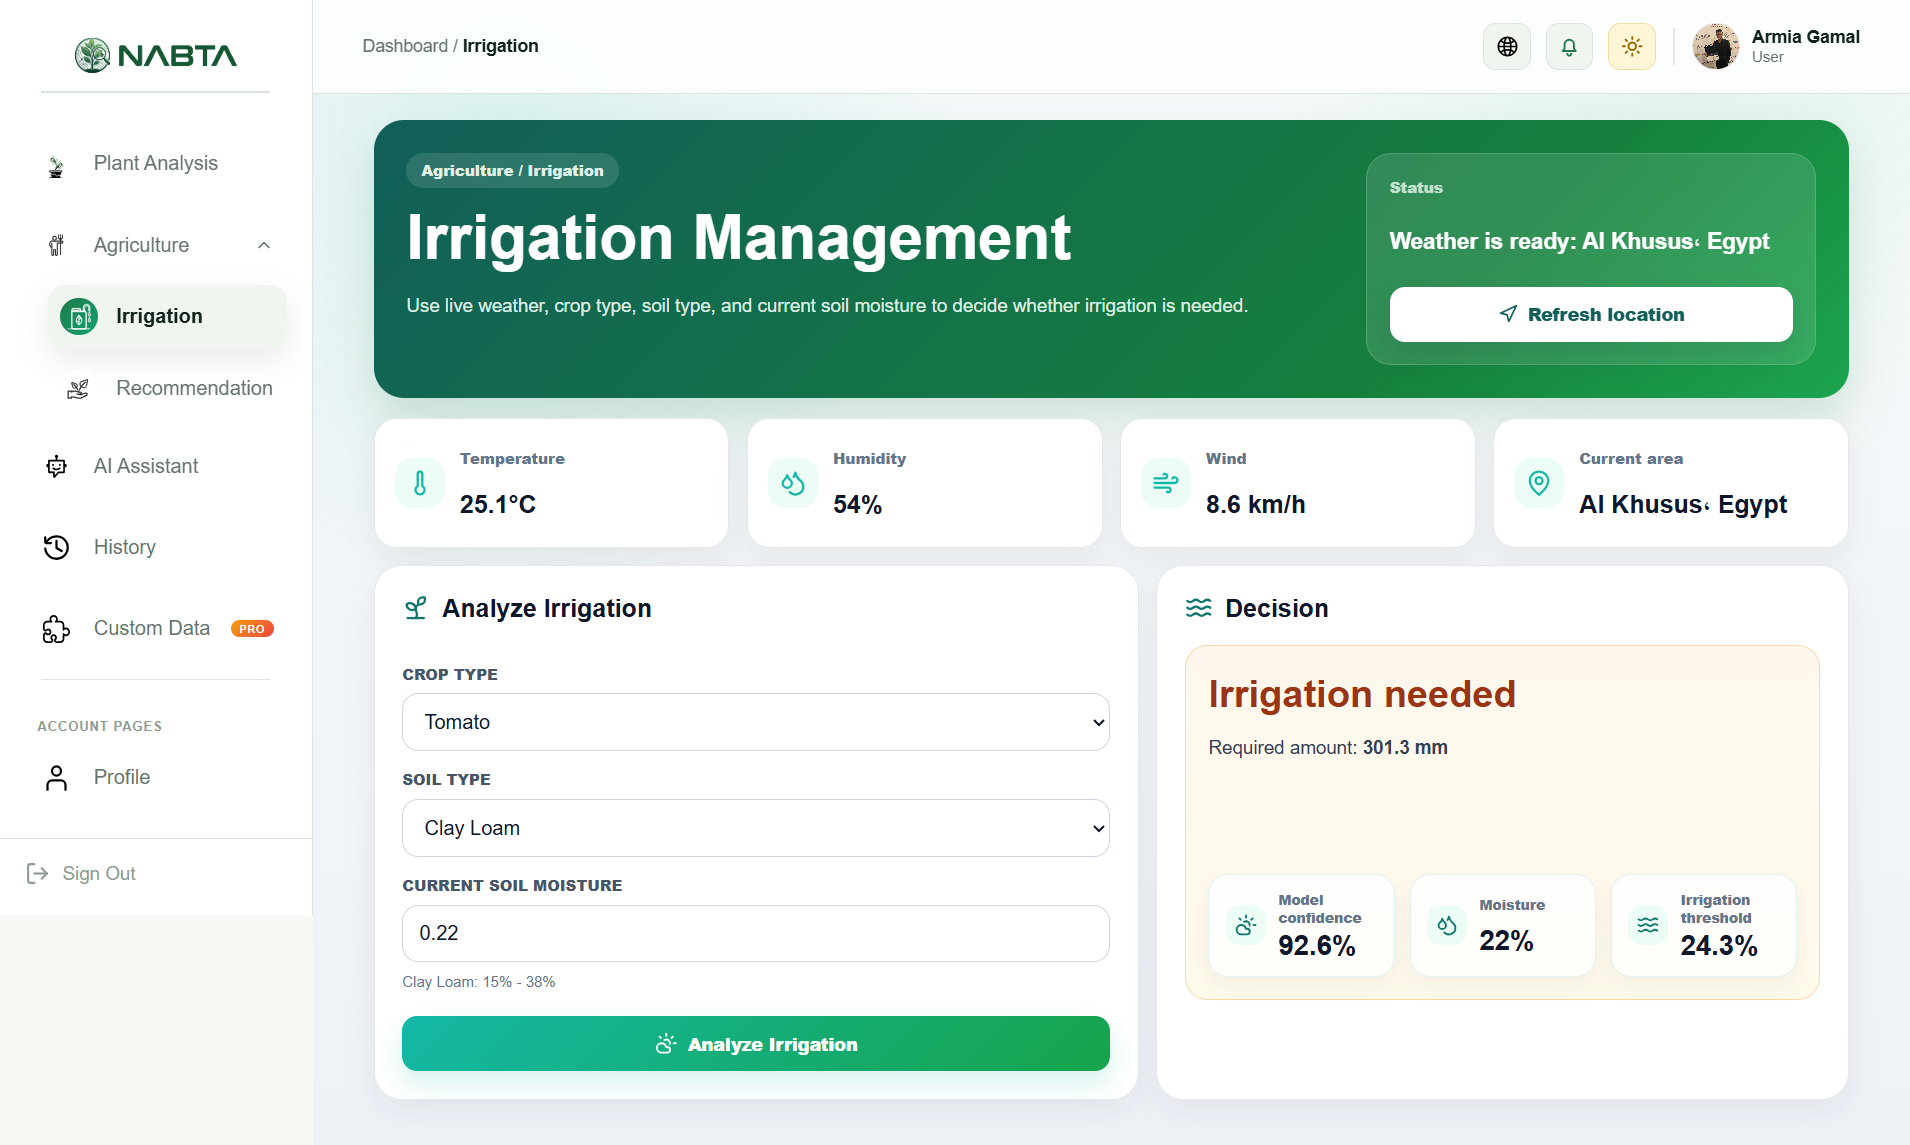
\includegraphics[width=\textwidth]{assets/screenshots/irrigation_management.png}
\caption{Smart Irrigation Management Interface}
\label{fig:irrigation}
\end{figure}

%==============================================================================
\subsection{Crop Recommendation}
\label{subsec:crop}

The crop recommendation module suggests the most suitable crop based on soil properties and environmental conditions.

Users enter the available Nitrogen (N), Phosphorus (P), Potassium (K), soil type, pH, temperature, humidity, and rainfall values. These inputs are processed by a Random Forest classifier trained on a regenerated agricultural dataset incorporating crop--soil suitability knowledge.

The system predicts the most appropriate crop together with confidence scores, allowing users to select crops that best match the current environmental conditions.

\begin{figure}[H]
\centering
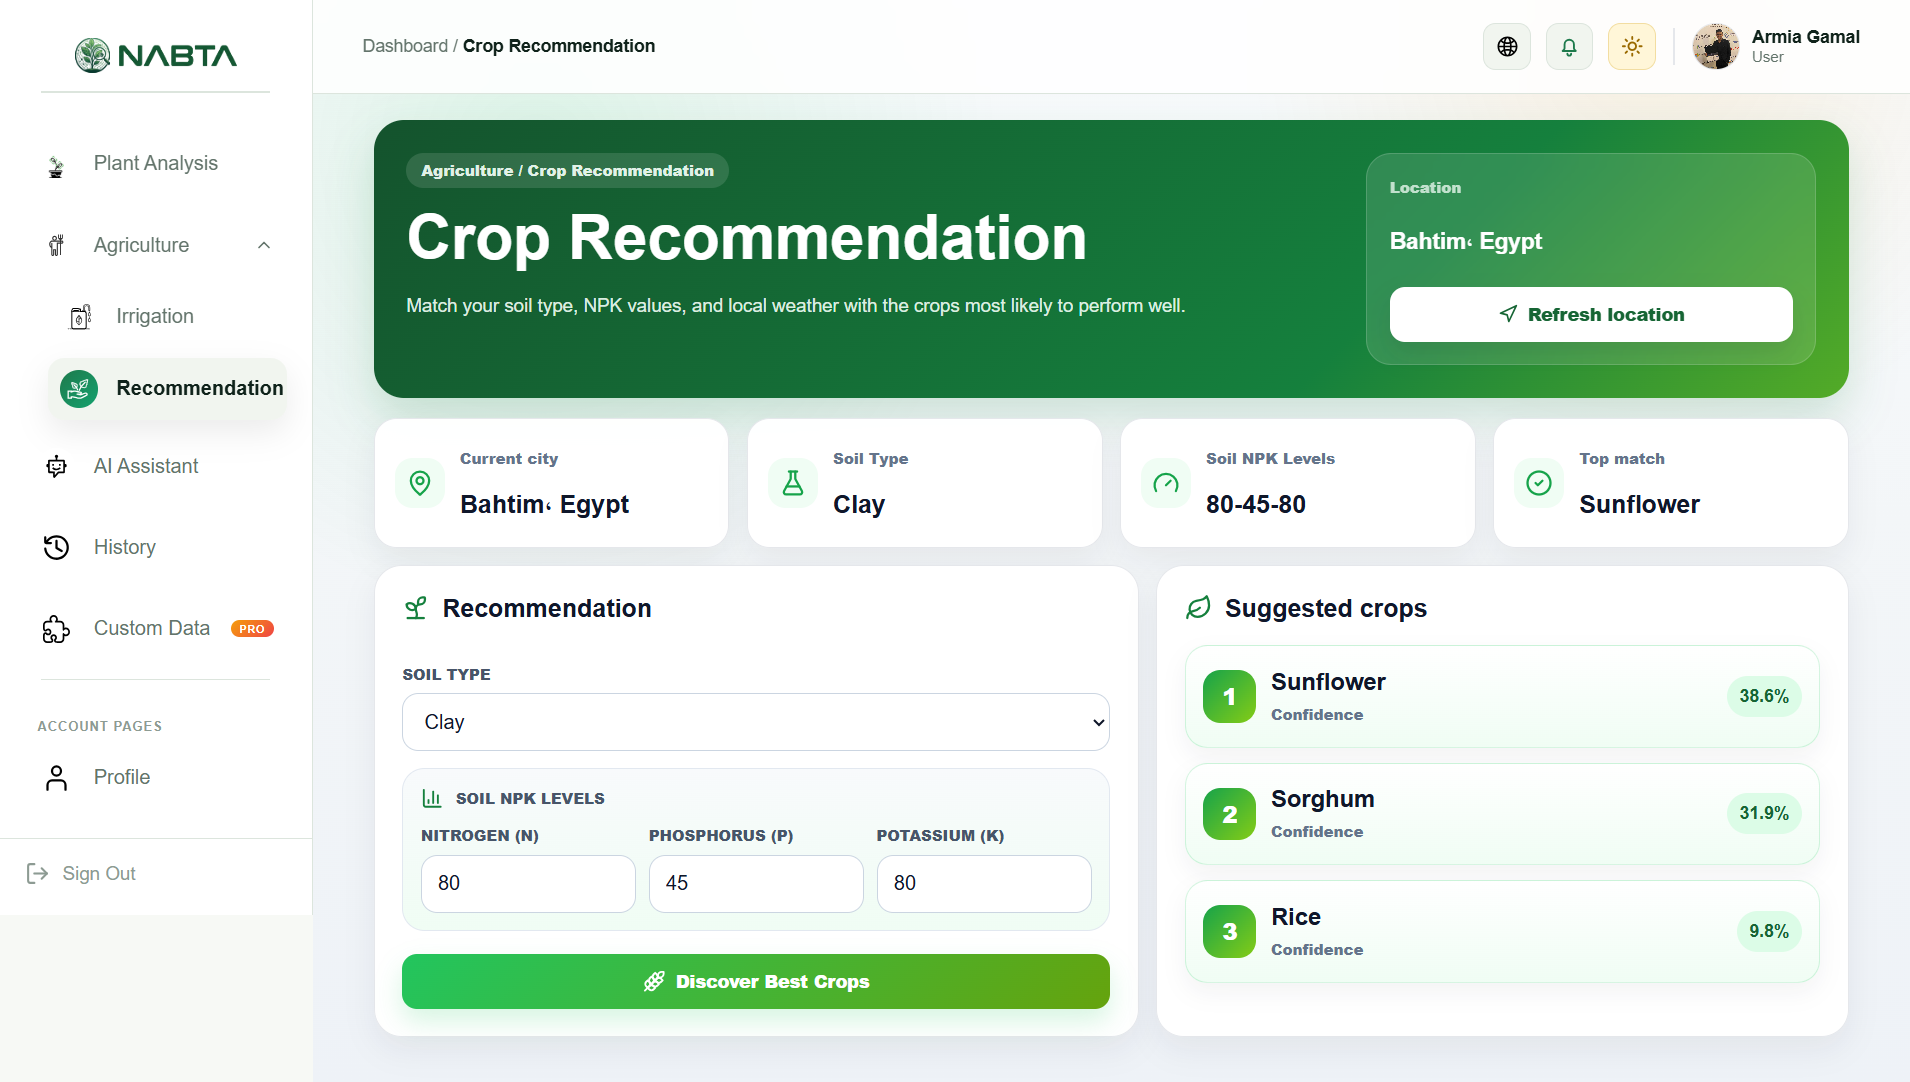
\includegraphics[width=\textwidth]{assets/screenshots/crop_recommendation.png}
\caption{Crop Recommendation Interface}
\label{fig:crop}
\end{figure}

%==============================================================================
\subsection{Custom Data Management}
\label{subsec:custom_data}

The platform includes a custom data management module that allows administrators to manage agricultural knowledge and user-generated data.

Authorized users can create, update, delete, and organize custom records through an intuitive interface. This functionality enables continuous expansion of the agricultural knowledge base while maintaining data consistency across the platform.

The management interface simplifies dataset maintenance without requiring direct database access.

\begin{figure}[H]
\centering
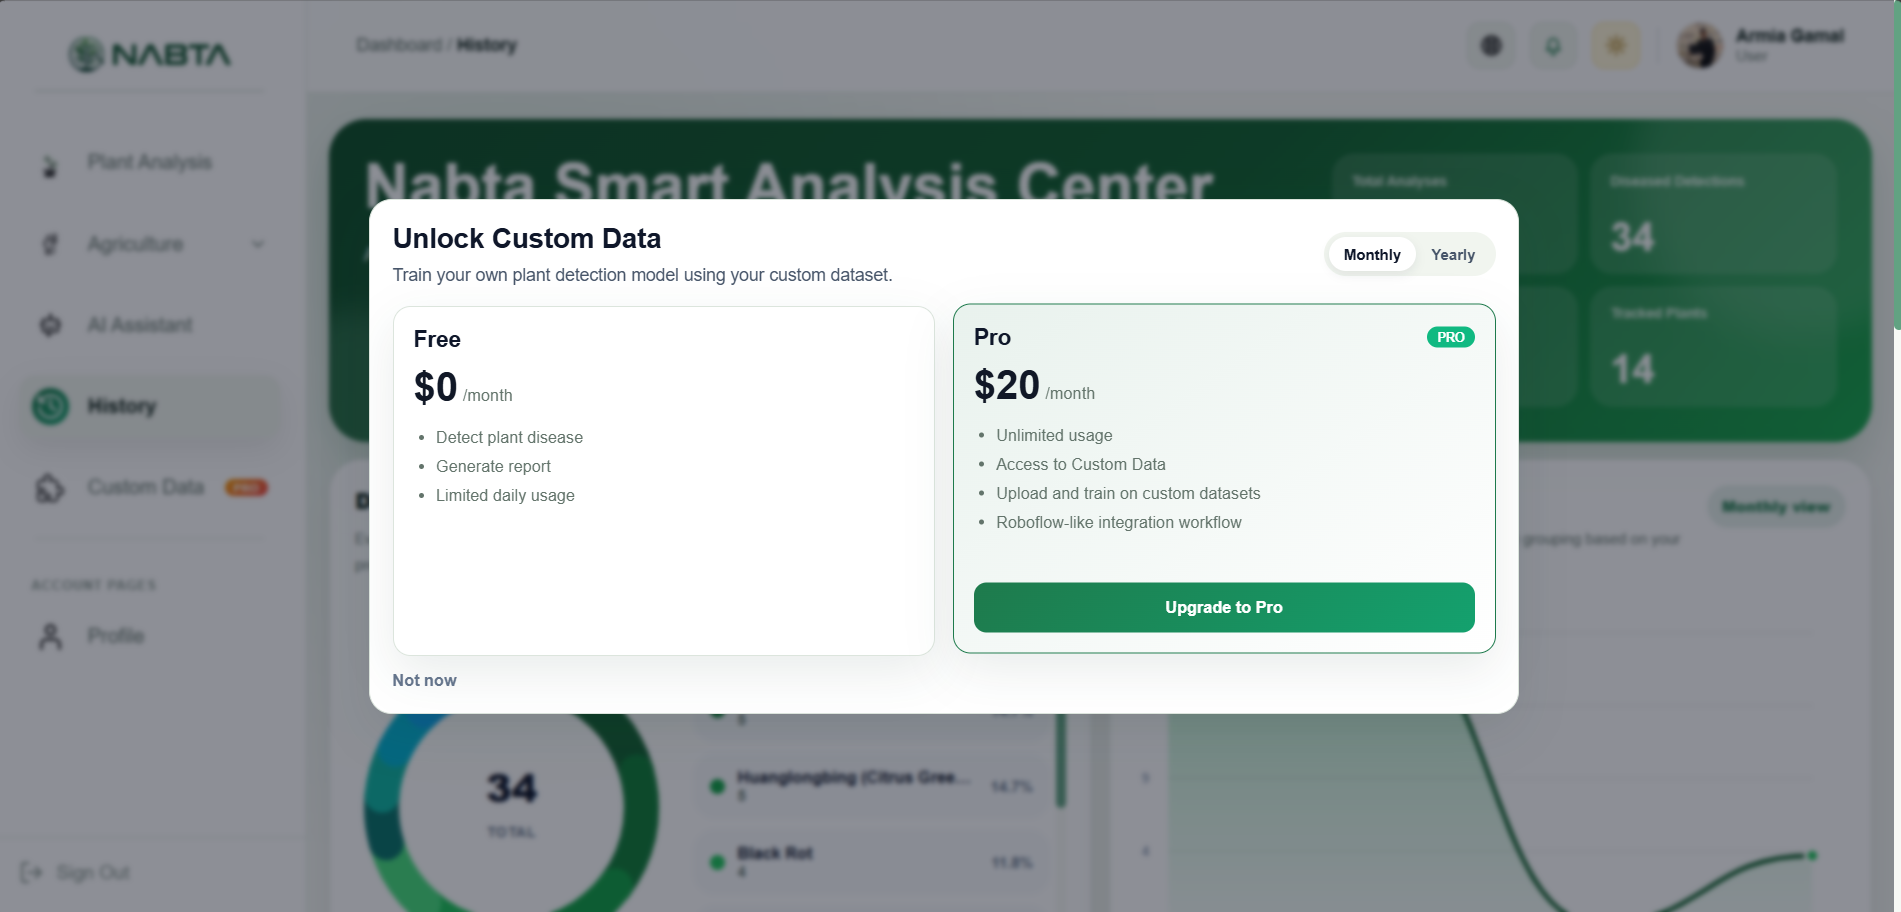
\includegraphics[width=\textwidth]{assets/screenshots/custom_data_management.png}
\caption{Custom Data Management Interface}
\label{fig:custom_data}
\end{figure}

%==============================================================================
\subsection{User Profile}
\label{subsec:profile}

Each registered user has a personalized profile containing account information, analysis statistics, generated reports, and personal preferences.

The profile page allows users to update personal information, change passwords, manage profile settings, and review their overall activity within the platform.

This centralized profile improves personalization while providing quick access to frequently used services.

\begin{figure}[H]
\centering
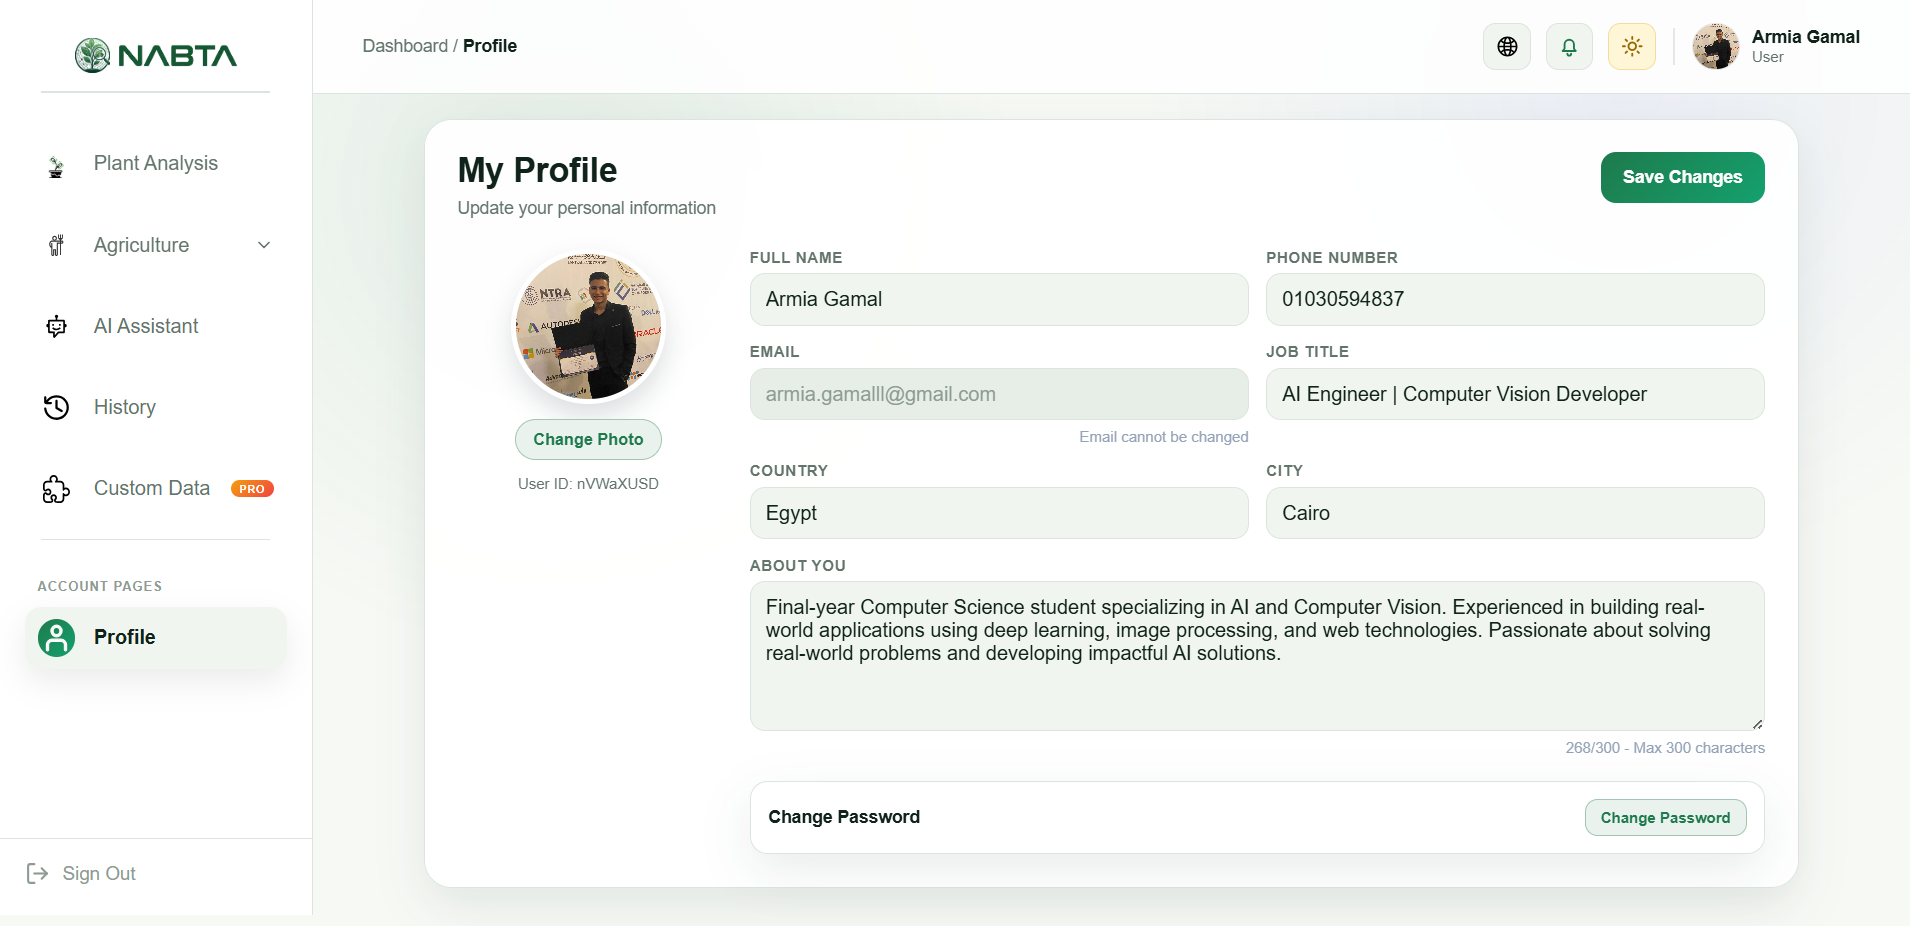
\includegraphics[width=\textwidth]{assets/screenshots/user_profile.png}
\caption{User Profile Interface}
\label{fig:profile}
\end{figure}

%==============================================================================
\section{Backend Implementation}
\label{sec:backend}

The backend of NABTA was implemented using FastAPI, providing a lightweight and high-performance RESTful API architecture.

FastAPI coordinates communication between the frontend, artificial intelligence models, Firebase services, and external APIs. The backend is responsible for image processing, model inference, authentication, report generation, chatbot interaction, and database communication.

Asynchronous request handling enables multiple users to access AI services simultaneously while maintaining low response latency.

%==============================================================================
\section{Artificial Intelligence Integration}
\label{sec:ai_integration}

One of the primary objectives of NABTA is the seamless integration of multiple artificial intelligence models within a single production-ready platform.

The AI pipeline consists of:

\begin{itemize}
\item YOLOv8x for infected leaf detection.
\item U-Net with EfficientNet-B0 encoder for semantic segmentation.
\item Custom CNN for disease classification.
\item Grad-CAM for explainability and disease severity estimation.
\item Random Forest classifier for crop recommendation.
\item Random Forest classifier for irrigation decision prediction.
\item Random Forest regressor for crop water requirement estimation.
\item Cohere Large Language Model integrated with Retrieval-Augmented Generation for intelligent agricultural consultation.
\end{itemize}

All models communicate through standardized FastAPI endpoints, enabling independent deployment while maintaining seamless integration across the entire platform.

%==============================================================================
\section{Cloud Services Integration}
\label{sec:firebase}

Firebase provides the cloud infrastructure supporting authentication, secure data storage, and backend services.

The platform utilizes Firebase Authentication for secure user management, Cloud Firestore for storing analysis history and user information, and Cloud Functions for backend automation, email notifications, and secure API operations.

These cloud services improve scalability, reliability, and security while minimizing infrastructure management overhead.

%==============================================================================
\section{Chapter Summary}
\label{sec:chapter4_summary}

This chapter presented the implementation of the NABTA smart agriculture platform, including the frontend interfaces, backend services, artificial intelligence integration, and cloud infrastructure.

The implementation demonstrates how multiple AI technologies were successfully combined into a unified web-based application that supports plant disease diagnosis, crop recommendation, irrigation management, explainable artificial intelligence, PDF report generation, and intelligent agricultural consultation.

The following chapter presents the experimental evaluation and performance analysis of all implemented artificial intelligence models.
